
\subsection{Illustration}
\label{sec:exps}

To illustrate our theoretical results, we evaluate the predictive performance and the ability of the models to capture homophily and preferential attachment on artificial and real networks. For homophily, we simply compare the distributions of the natural and latent similarities on linked and non-linked pairs of nodes. For global preferential attachment, we use plots of the degree distribution and its corresponding best fitting line in log-log scale. In addition, we use the measure developed in \cite{clauset2009power} for assessing whether empirical data behaves according to a power law (as mentioned before, power laws are the standard bursty distributions in social networks \cite{barabasi1999emergence}). This framework combines maximum-likelihood methods with goodness-of-fit tests based on the Kolmogorov-Smirnov statistics to compute a $p$-value. If the obtained $p$-value is large (close to 1), then the data is likely to be distributed according to a power law and the associated network displays preferential attachment;  on the other hand, if it is small, the data is likely not distributed according to a power law and the associated network does not display preferential attachment.

For local preferential attachment, we follow the same approach as before to compute the $p$-value, the only difference being that the empirical data does not correspond any longer to the global adjacency matrix, but to reduced matrices for each class. The computation of the reduced adjacency matrices varies from one model to the other:
%
\begin{itemize}
    \item For \imb, for a given class $k$, the reduced adjacency matrix $Y^k$ is defined by:~$y_{ij,k}=1$ if $y_{ij}=1, z_{i\rightarrow j}=z_{i\leftarrow j}=k$ and $0$ otherwise.
    \item For \ifm, the reduced adjacency matrix $Y^k$ is defined by:~$ y_{ij,k}=1$ if $y_{ij}=1 , f_{ik}=f_{jk}=1$ and $0$ otherwise.
\end{itemize}~\\


Note that all our experiments where realized in a platform that we developed and maintain in order to help reproducibility of machine learning experiments. It is available online \footnote{https://github.com/dtrckd/pymake} under a GNU GPL license.

\subsection{Datasets and model parameters}

To illustrate the above developments, we consider two artificial and two real networks, the characteristics of which are summarized in Table~\ref{table:networks_measures}.


\begin{table}[h] {Characteristics of artificial and real networks.}
    \begin{tabular}{lrrr}
        \hline
        \textbf{Networks} &   nodes &   edges &   density \\
        \hline
        Network1 &    1000 &    3507 &     0.007 \\
        Network2 &    1000 &   31000 &     0.062 \\
        Blogs         &    1490 &   20512 &     0.009 \\
        Manufacturing &     167 &    5950 &     0.215 \\
    \hline
    \end{tabular}
	\label{table:networks_measures}
\end{table}



The non-oriented artificial networks (Network1 and Network2) have been generated with the DANCer-Generator \cite{largeron2015}. This generator has been chosen because it allows one to build an attributed graph having a community structure as well as known properties of real-world networks such as preferential attachment and homophily. In order to test link prediction models on different types of networks, Network1 was generated, by design, to comply with preferential attachment whereas Network2 was not.

The first real network, denoted Blogs \footnote{moreno.ss.uci.edu/data.html\#blogs}, contains front-page hyperlinks between blogs in the context of the 2004 US election. A node represents a blog and an oriented link represents a hyperlink between two blogs. The second one, denoted Manufacturing \footnote{www.ii.pwr.edu.pl/~michalski/index.php?content=datasets\#manufacturing}, is an internal email communication network between employees of a mid-sized manufacturing company. Each node is associated to an employee and an oriented link represents an email sent between the two employees. One can notice that the second network is specific since it is an enterprise network in which the relationships between the employees are (professionally) constrained. This means that this network is less likely to display some of the properties that occur in unconstrained social networks.

The adjacency matrices and global degree distributions of these networks are presented in Figure \ref{fig:corpuses}. The adjacency matrices enable us to visualize some characteristics of the networks such as their density and their clustering patterns: as one can note, Blogs and the two artificial networks (Network1 and Network2) have a clear community structure, corresponding to the blocks of white dots on the figure, whereas Manufacturing, the denser network, does not have such a structure. Furthermore, the log-log scale plots show that Network1 and Blogs verify the  global preferential attachment (the fitted line represents relatively well the data points) whereas neither Network2 nor Manufacturing verify it. This is confirmed by the $p$-values reported in the first section of Table \ref{table:me_gofit} (Training Datasets): the $p$-value is 1 for Network1 and Blogs, whereas it is null for Network2 and Manufacturing. The parameter $\alpha$ reported in Table~\ref{table:me_gofit} corresponds to the parameter of the estimated power law distribution (\textit{i.e.} the slope of the best fitting line in log-log scale).

Figure \ref{fig:synt_graph_local} represents the local degree distributions for all networks, each curve in each plot being associated to a different class. As the ground truth is not available for the real networks (Blogs and Manufacturing), classes have been determined with Louvain algorithm \cite{Blondel2008} and the local distribution defined according to the obtained classes. As one can note, the plots for Network1 and Blogs are linear for the most frequent degrees, whereas the plots for Network2 and Manufacturing do not display any clear linearity, suggesting that Network1 and Blogs satisfy, at least partly, local preferential attachment whereas Network2 and Manufacturing do not. This is confirmed by the $p$-values reported in Table~\ref{table:me_gofit}: the $p$-value equals  $1$ for Network1 and Blogs,  $0$ for Network2 and $0.4$ for Manufacturing.

\begin{figure}[ht!]
    \centering
        \begin{minipage}{0.4\textwidth}
            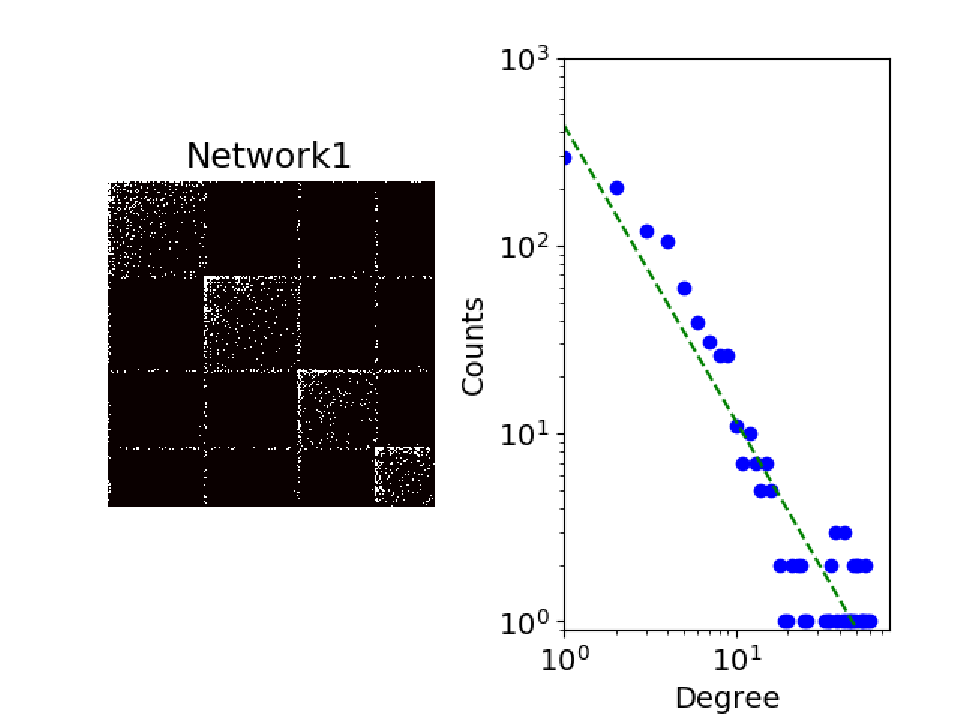
\includegraphics[width=\textwidth]{img/corpus/network1_dd}
        \end{minipage}
        \begin{minipage}{0.4\textwidth}
            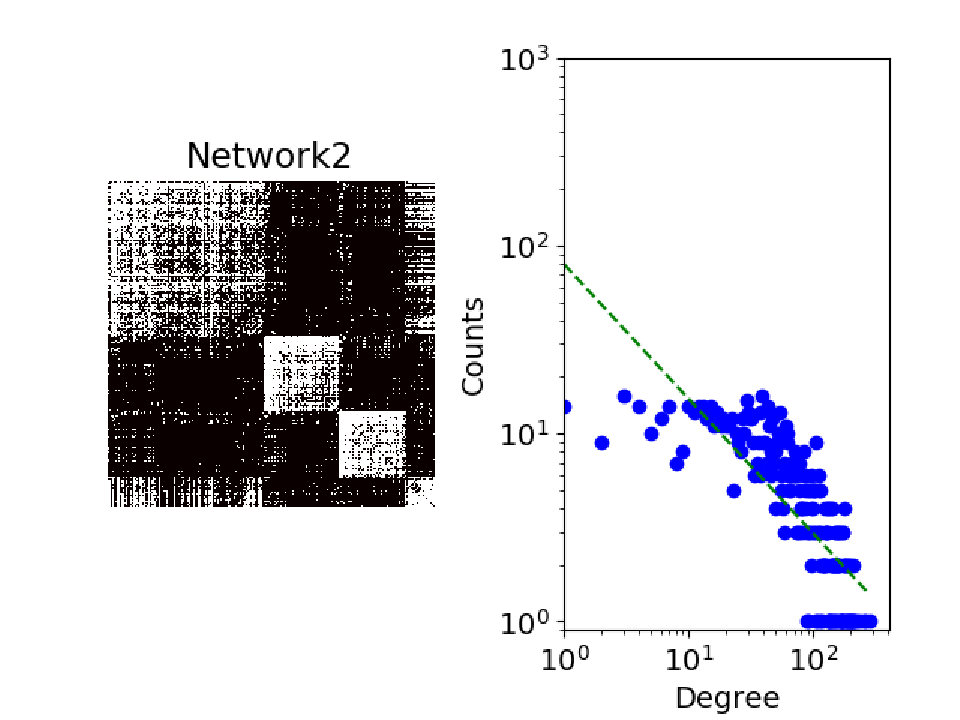
\includegraphics[width=\textwidth]{img/corpus/network2_dd}
        \end{minipage}
        %\vskip\baselineskip
        \begin{minipage}{0.4\textwidth}
            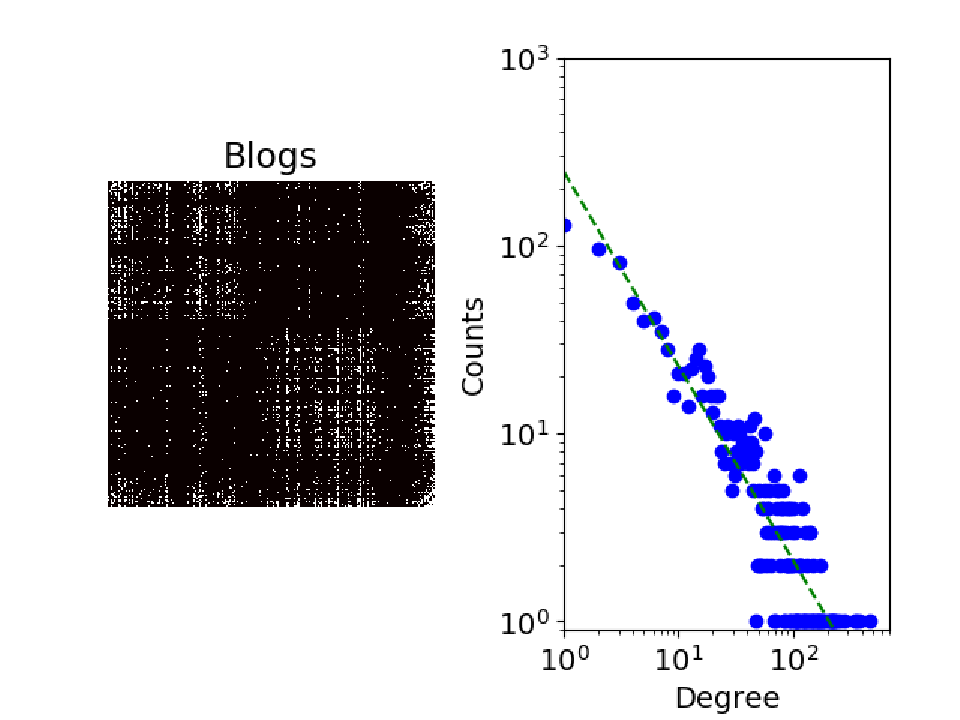
\includegraphics[width=\textwidth]{img/corpus/blogs_dd}
        \end{minipage}
        \begin{minipage}{0.4\textwidth}
            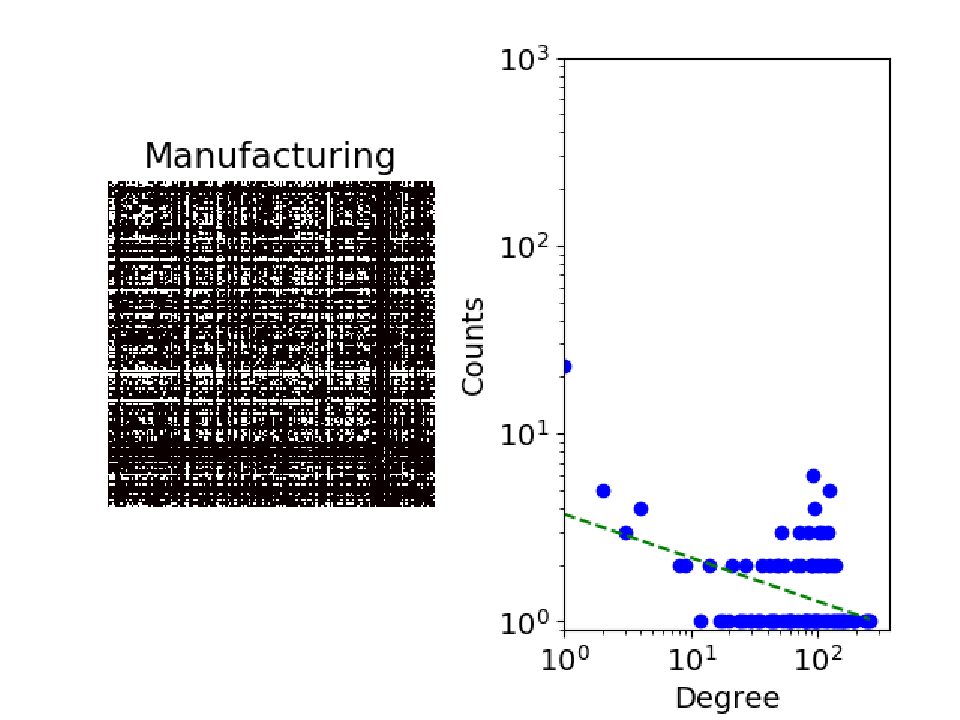
\includegraphics[width=\textwidth]{img/corpus/manufacturing_dd}
        \end{minipage}
	\caption{Adjacency matrices (left) and global degree distributions (right) for the four training datasets. In the adjacency matrices, a white dot corresponds to a 1 and a black dot to a 0.}
	\label{fig:corpuses}
\end{figure}

\begin{figure}[h]
    \centering
        \begin{minipage}{0.4\textwidth}
            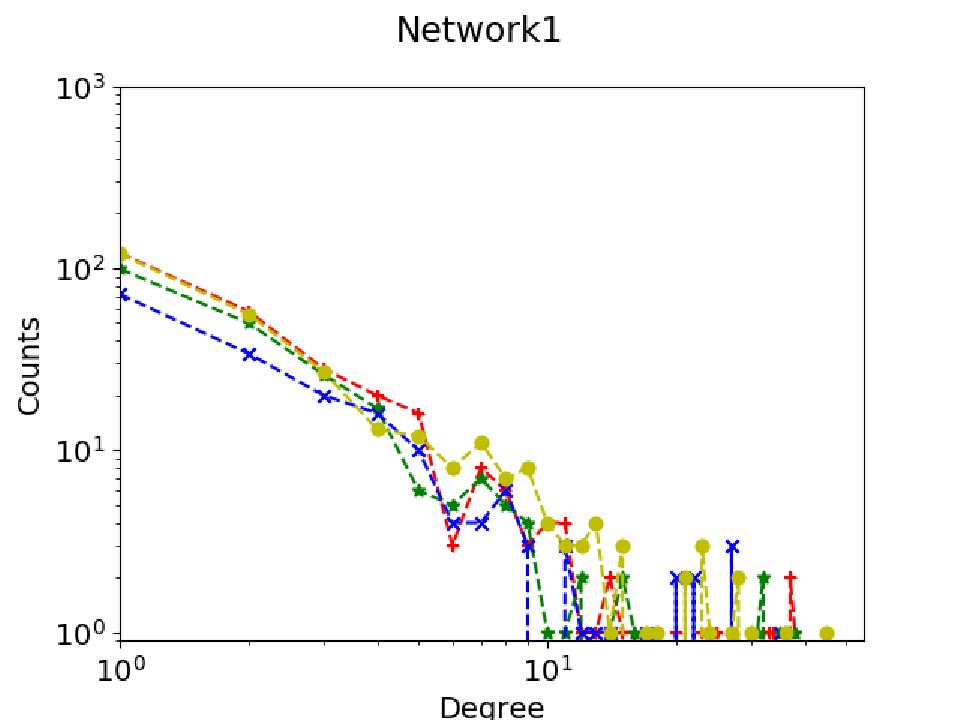
\includegraphics[width=\textwidth]{img/corpus/network1_1}
        \end{minipage}
        \begin{minipage}{0.4\textwidth}
            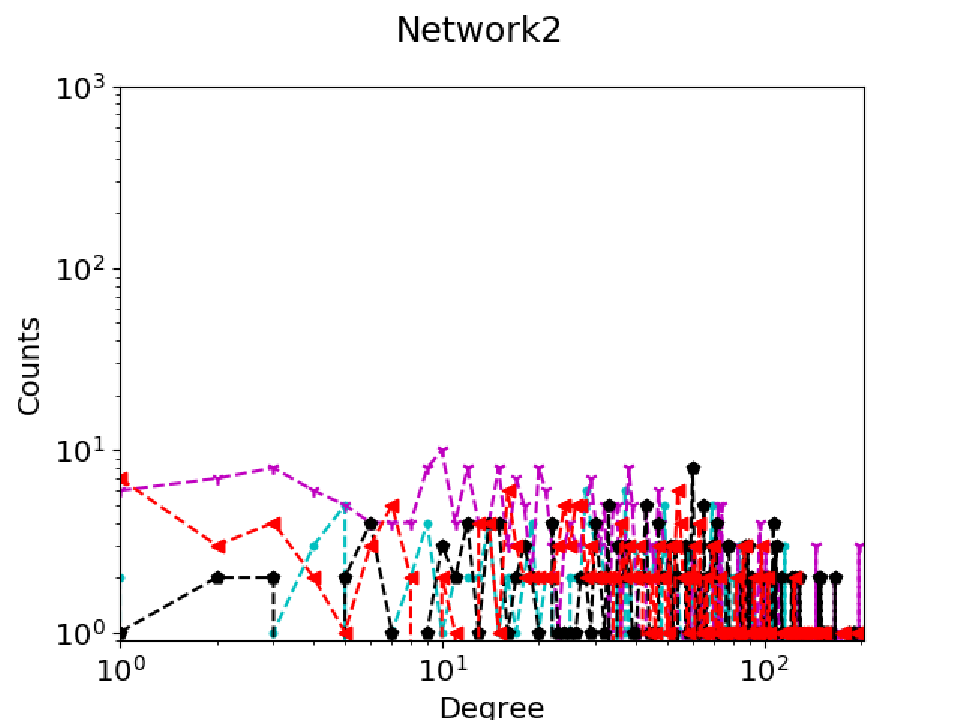
\includegraphics[width=\textwidth]{img/corpus/network2_1}
        \end{minipage}
        \vskip\baselineskip
        \begin{minipage}{0.4\textwidth}
            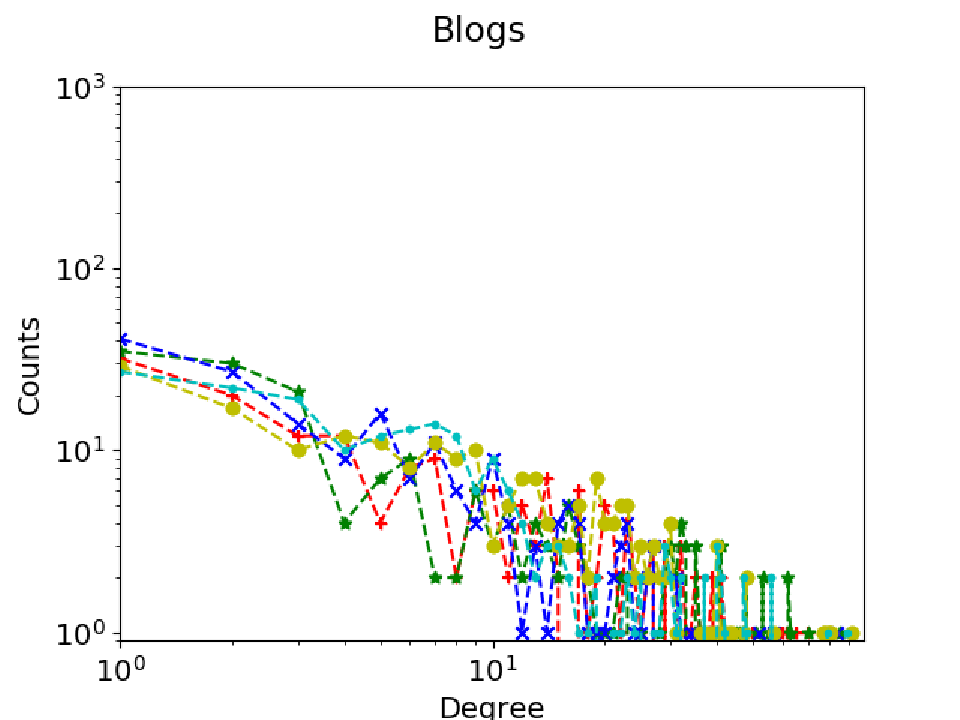
\includegraphics[width=\textwidth]{img/corpus/blogs_1}
        \end{minipage}
        \begin{minipage}{0.4\textwidth}
            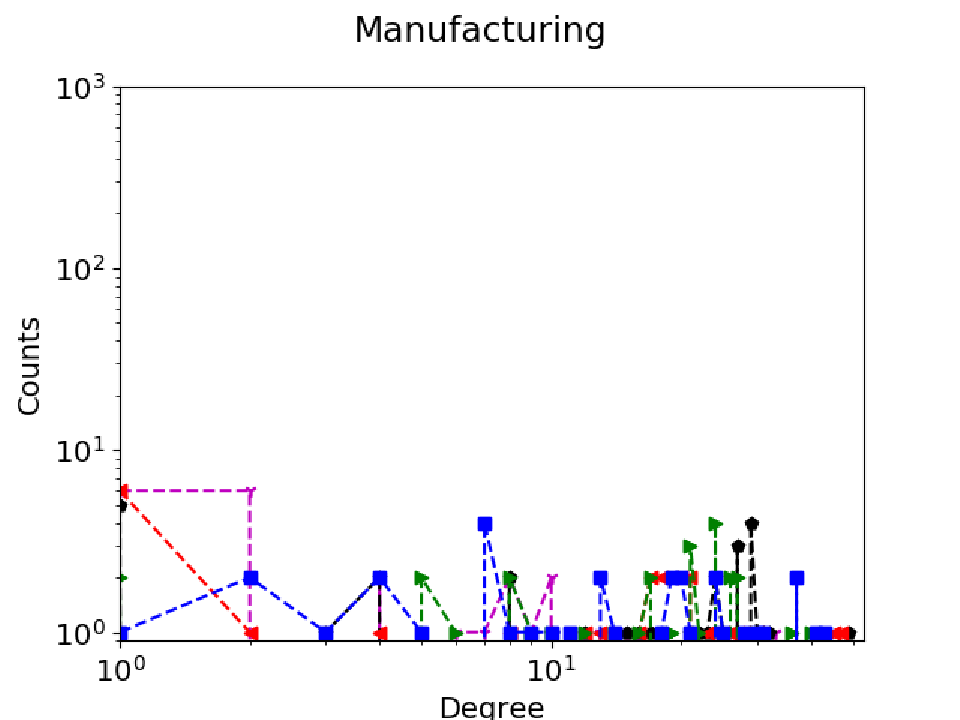
\includegraphics[width=\textwidth]{img/corpus/manufacturing_1}
        \end{minipage}
        \caption {Local degree distributions for the four training datasets. For Network1 and Network2 the classes come from ground-truth. For Blogs and Manufacturing, classes are obtained by Louvain algorithm.} 
	\label{fig:synt_graph_local}
\end{figure}

For each dataset, we estimate the model parameters through Markov Chain Monte Carlo inference consisting of 200 iterations. For \imb, the concentration parameters of HDP were optimized  using vague gamma priors $\alpha_0 \sim \text{Gamma}(1,1)$ and $\gamma \sim \text{Gamma}(1,1)$ following \cite{HDP}. The parameters for the matrix weights  $\lambda_0$ and $\lambda_1$ were fixed to 0.1. For \ifm, the hyperparameter  $\sigma_w$ was fixed to 1 and the IBP hyperparameter $\alpha$ to 0.5 in order to  have comparable number of classes with \imb. Once the models have been learned, they are used to generate links (or non-links) between the entire set of network nodes. The whole procedure is repeated 10 times and the average values are reported as final results.

\subsection{Homophily}

Figure \ref{fig:homo_mustach} presents boxplots describing the distributions of the natural $s_n(i,j)$ and latent $s_l(i,j)$ similarities computed respectively on linked and non-linked pairs of nodes for \imb\ (top) and \ifm\ (bottom). The results have been aggregated over the four datasets. They confirm that the natural similarity is  higher for pairs of nodes which are linked than for pairs of nodes which are not linked, for both models. For the latent similarity,  there is no difference between the linked and non-linked pairs, indicating that the links are not homophilic. These experimental results are in line with the theoretical results presented in Section~\ref{sec:homophily} that state that both \ifm\ and \imb\ are homophilic for  the natural similarity but are not homophilic for the latent similarity.

\begin{figure}[ht]
\centering
    \begin{subfigure}
       	 \centering
        	 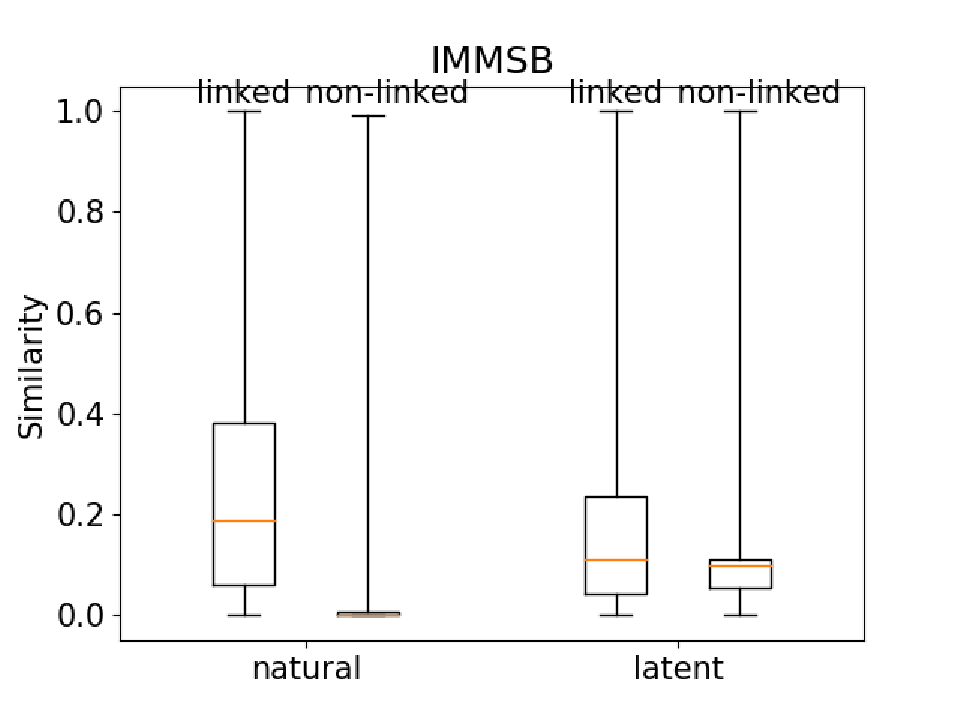
\includegraphics[width=0.38\textwidth]{img/corpus/homo_mustach_immsb}
    \end{subfigure}
    \begin{subfigure}
        	 \centering
          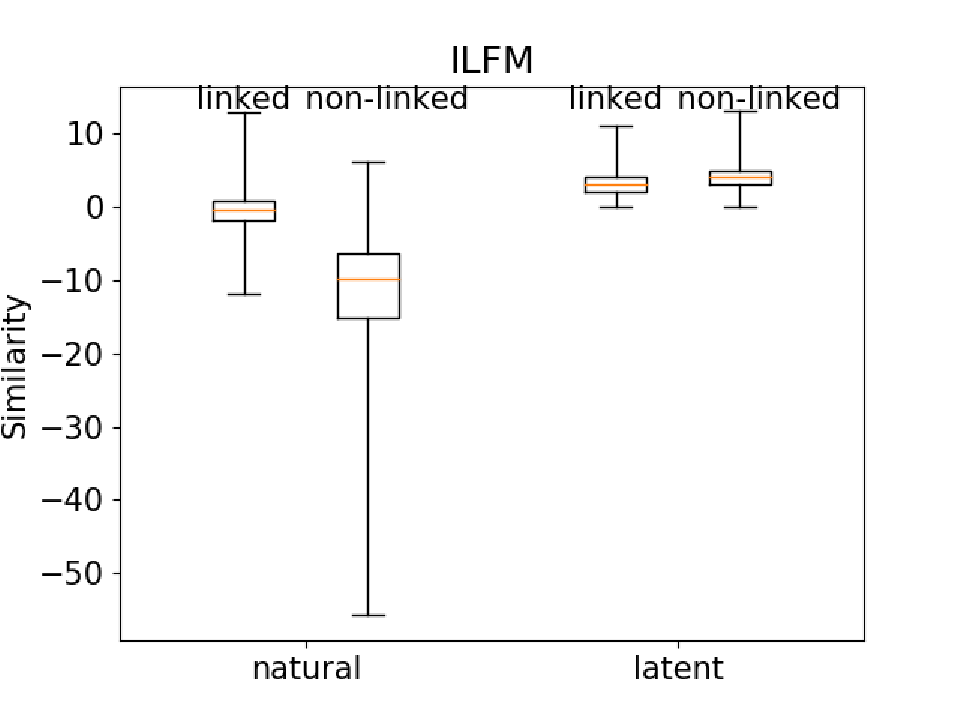
\includegraphics[width=0.38\textwidth]{img/corpus/homo_mustach_ilfm}
    \end{subfigure}
    \caption{Natural and latent similarities aggregated over all datasets and computed on linked and non-linked pairs of nodes for \imb\ (top) and \ifm\ (bottom).}
    \label{fig:homo_mustach}
\end{figure}

\subsection{Preferential attachment}

Table \ref{table:me_gofit} reports the value of the power-law goodness of fit for \imb\ and \ifm\ in the global case (left) and in the local case (right). It appears that for both models, the global preferential attachment is only verified for networks generated from datasets where the property was observed, namely in Network1 with p-value equal to 0.9 for \imb\ and 1 for \ifm, and in Blogs with a p-value equal to 1 for both models; the property is not verified in Network2 and in Manufacturing, where p-values are equal to 0. This is in accordance with Proposition 2.1 according to which both \ifm\ and \imb\ do not satisfy global preferential attachment. However, these models are able to capture this property if it exists in the training datasets.  Moreover, one can observe that, in the local case, \imb\ complies with the preferential attachment with $p$-values equal or close to 1 for the four networks, while \ifm\ obtained low p-values for the networks that were less locally bursty (respectively  0  for Network2 and 0.3 for Manufacturing). In addition, the power-law coefficients $\alpha$ are significantly greater for \imb\ than for \ifm, and specially for the bursty networks Network1 and Blogs.

Figure \ref{fig:me_local} illustrates the local preferential attachment for Network1 (top) and Network2 (bottom) estimated with \imb\ (left) and \ifm\ (right). The shape of the local degree distributions appears more linear for \imb\ and with more fluctuations for \ifm. This illustrates the fact that \ifm\ does not capture local preferential attachment whereas \imb\ does, as stated in Proposition 2.2. 


\begin{table}[h]{Preferential attachment measures for training datasets and networks generated with fitted models.}
\begin{tabular}{lrrrr}
  \multirow{2}{*}{\textbf{Training Datasets}}  &
  \multicolumn{2}{c}{Global} & \multicolumn{2}{c}{Local}\\
  \cmidrule(r){2-3} \cmidrule(l){4-5}
  &   $p$-value &   $\alpha$   & $p$-value & $\alpha$   \\
\hline
Network1       & 1 & 2.4 &   1.0 $\pm$ 0.0  &  1.8 $\pm$ 0.03  \\
Network2       & 0 & 1.3 &   0.0 $\pm$ 0.0  &  1.2 $\pm$ 0.01 \\
Blogs          & 1 & 1.5 &   1.0 $\pm$ 0.0  &  1.4 $\pm$ 0.03\\
Manufacturing  & 0 & 1.4 &   0.4 $\pm$ 0.3  &  1.3 $\pm$ 0.05 \\
\hline

  \ \textbf{\immsb} &&&& \\
\hline
Network1       & 0.9 & 1.4 &   1.0 \(\pm\) 0.0   &  3.5 \(\pm\) 0.7 \\
Network2       & 0 & 1.3 &   0.9 \(\pm\) 0.0   &  1.6 \(\pm\) 0.2 \\
Blogs          & 1 & 1.3 &   1.0 \(\pm\) 0.0   &  4.3 \(\pm\) 1.1 \\
Manufacturing  & 0 & 1.2 &   0.9 \(\pm\) 0.01  &  1.6 \(\pm\) 0.1 \\
\hline

  \ \textbf{\ilfm} &&&& \\
\hline
Network1      & 1 & 1.4 &   1.0 \(\pm\) 0.0  &  1.7 \(\pm\) 0.1 \\
Network2      & 0 & 1.2 &   0.0 \(\pm\) 0.0 &  1.2 \(\pm\) 0.0 \\
Blogs         & 1 & 1.3 &   0.9 \(\pm\) 0.2  &  1.5 \(\pm\) 0.1 \\
Manufacturing & 0 & 1.2 &   0.3 \(\pm\) 0.3  &  1.3 \(\pm\) 0.0 \\
\hline
\end{tabular}
\label{table:me_gofit}
\end{table}


\begin{figure}[h]
    \centering
    \begin{minipage}{0.4\textwidth}
        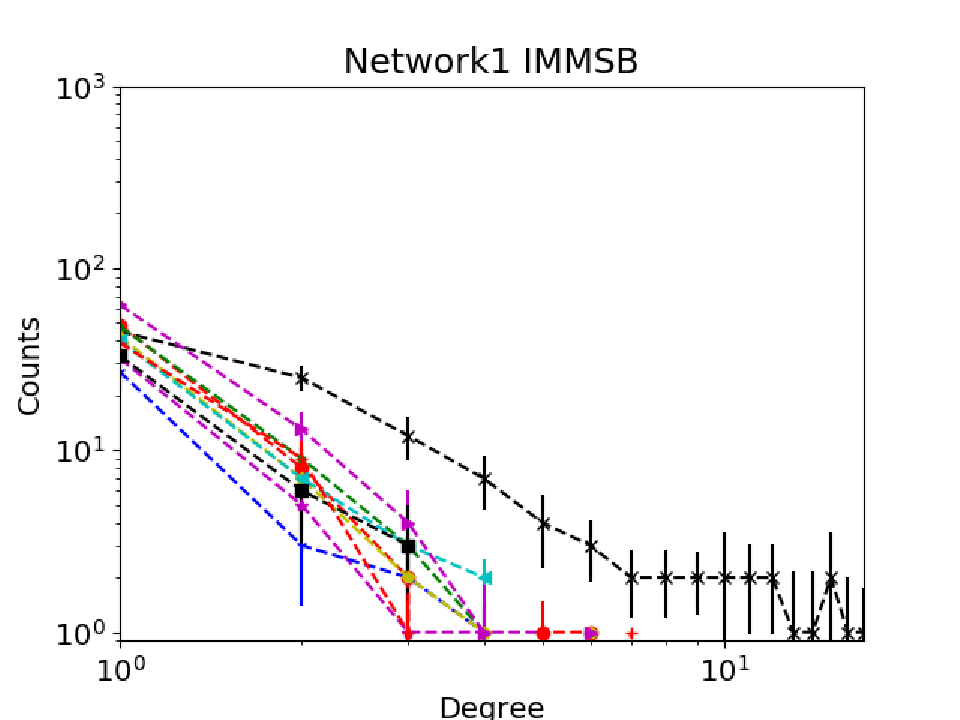
\includegraphics[width=\textwidth]{img/corpus/immsb_network1_1}
    \end{minipage}
    \begin{minipage}{0.4\textwidth}
        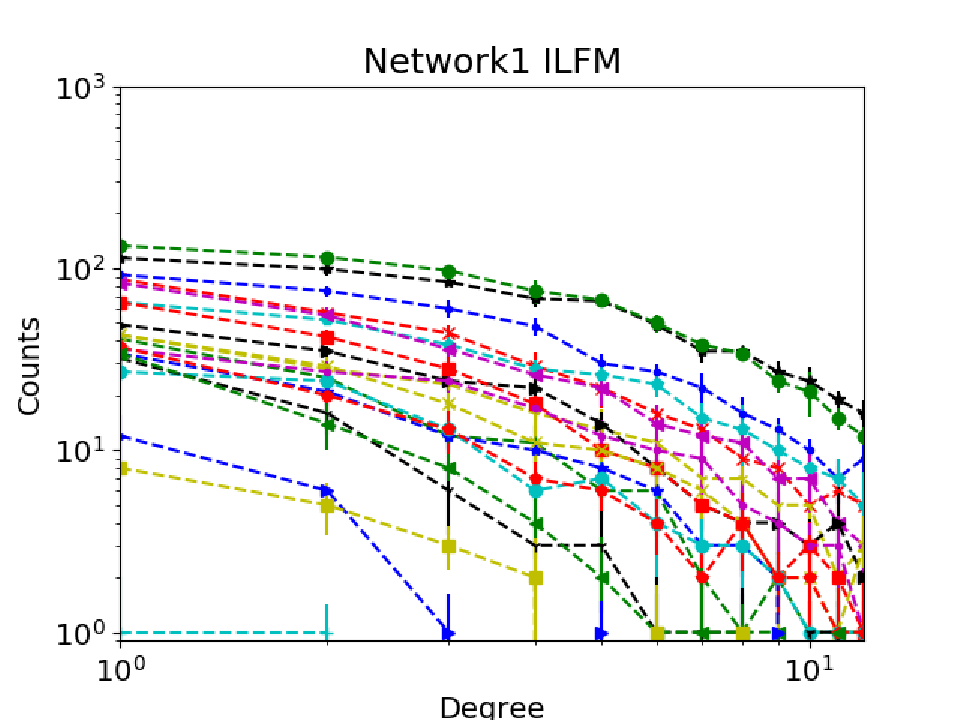
\includegraphics[width=\textwidth]{img/corpus/ilfm_network1_1}
    \end{minipage}
    \vskip\baselineskip
    \begin{minipage}{0.4\textwidth}
        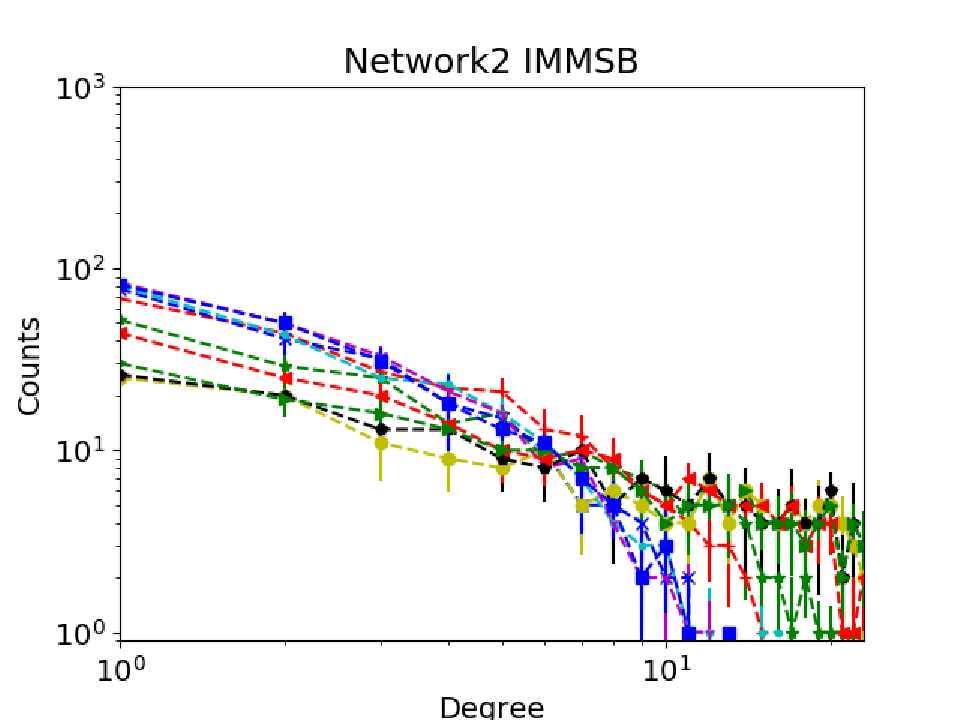
\includegraphics[width=\textwidth]{img/corpus/immsb_network2_1}
    \end{minipage}
    \begin{minipage}{0.4\textwidth}
        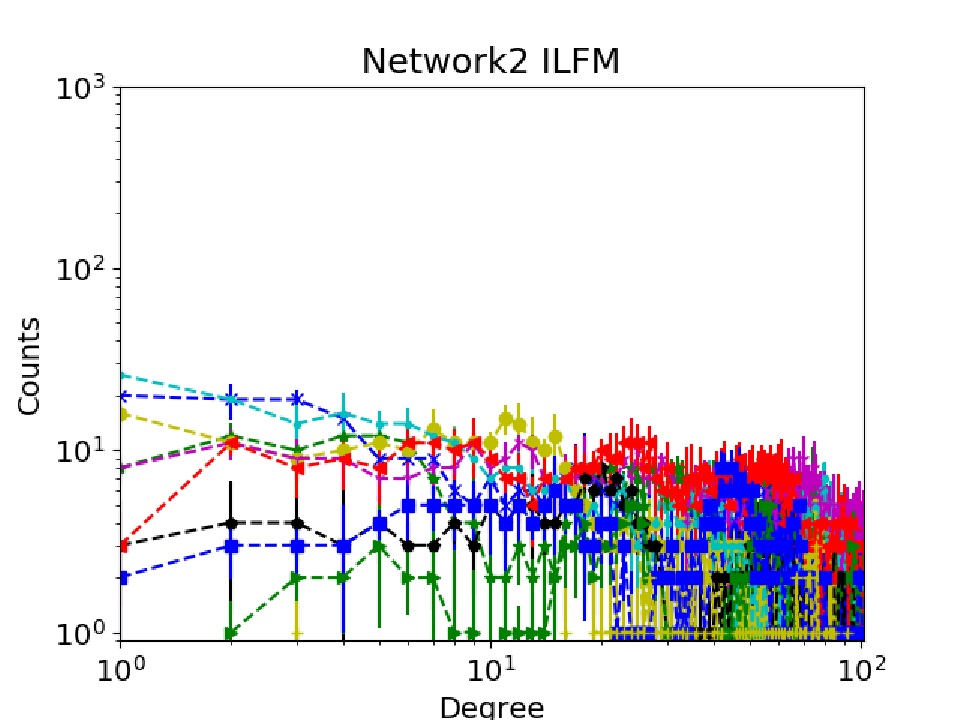
\includegraphics[width=\textwidth]{img/corpus/ilfm_network2_1}
    \end{minipage}
    \caption {Local degree distributions for Network1 (top row) and Network2 (bottom row) generated with fitted models \imb\ (first column) and \ifm\ (second column).} 
\label{fig:me_local}
\end{figure}

\begin{figure}[ht!]
\centering
    \begin{minipage}{0.4\textwidth}
        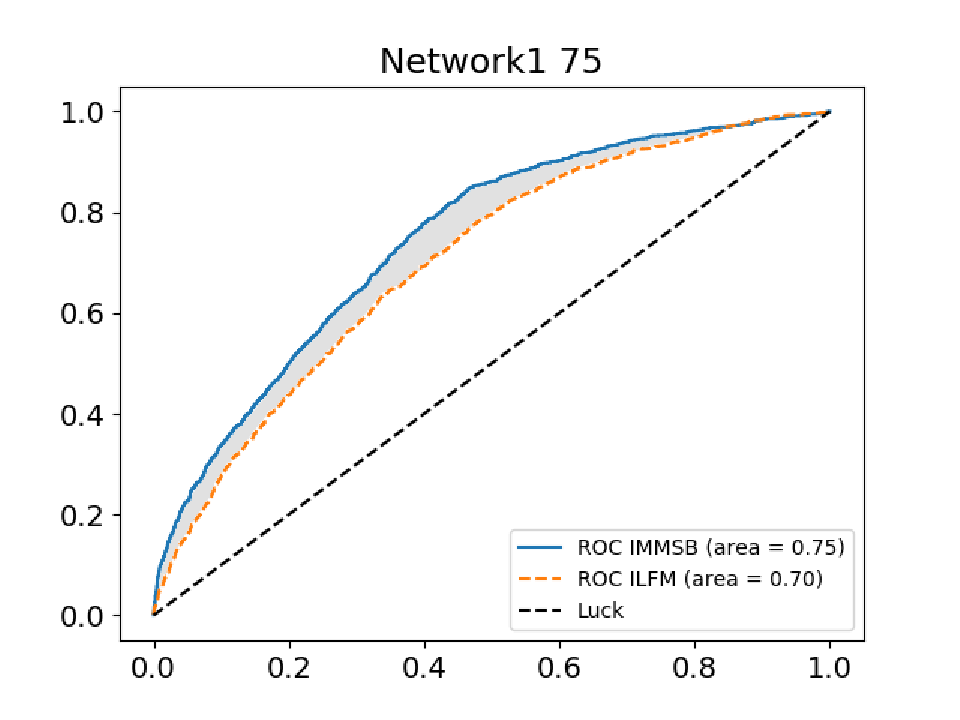
\includegraphics[width=\textwidth]{img/corpus/roc_network1_75_f}
    \end{minipage}
    \begin{minipage}{0.4\textwidth}
        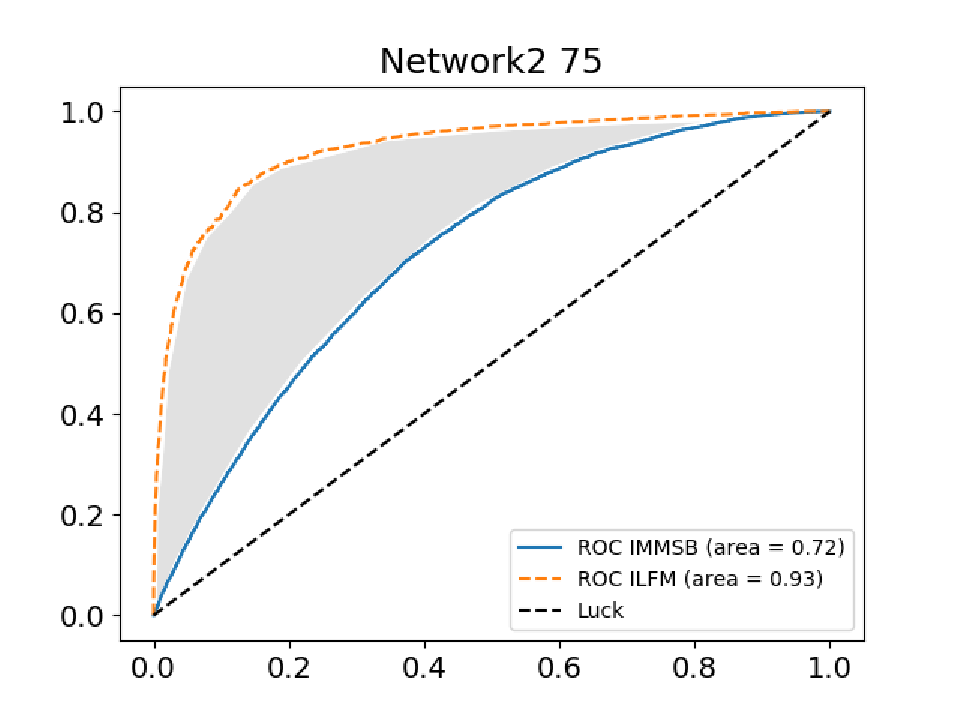
\includegraphics[width=\textwidth]{img/corpus/roc_network2_75_f}
    \end{minipage}
    \begin{minipage}{0.5\textwidth}
        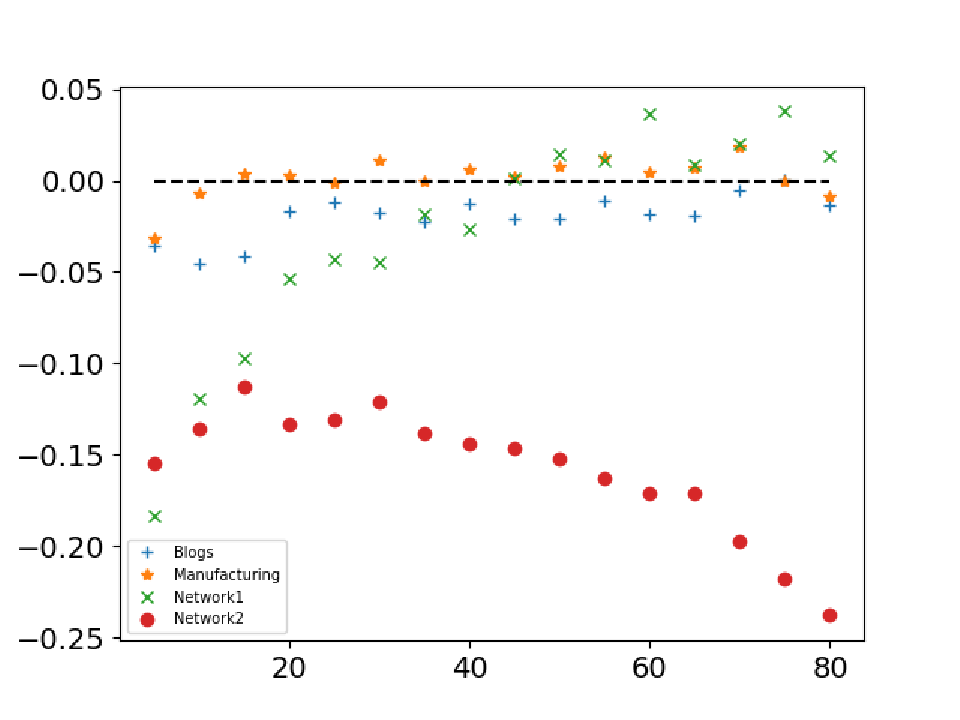
\includegraphics[width=\textwidth]{img/corpus/testset_max_20}
    \end{minipage}
    \caption{Top: AUC-ROC curves for Network1 (left) and Network2 (right) with 75 percent of data used for learning that compares the performance of models. Bottom: Relative performance of \imb\ and \ifm\ according to the percentage of data used for testing, the rest being used for learning; the number of training data decreases with the x-axis and a positive value on the y-axis indicates that \imb\ outperforms \ifm.} 
\label{fig:auc}
\end{figure}

Lastly, Figure \ref{fig:auc} compares the performance of the models for predicting new links using the Area Under the Curve (AUC) measure as a function of the training set size. In the bottom plot, the y-axis gives the relative performance defined as the difference of the AUC values for \imb\ and \ifm\ ($AUC_{\imb} - AUC_{\ifm}$) whereas the x-axis indicates the percentage of links randomly removed from the datasets and used as test examples. Hence, the number of training data decreases with the x-axis and a positive value on the y-axis indicates that \imb\ outperforms \ifm.  The relative performance corresponds to the difference of the MAX AUC values obtained for both models on the 10 inference experiences. The top plots illustrate a case where 75 percent of the data is used as test set and where \imb\ dominates \ifm\ on Network1 (left), and the opposite on Network2 (right).

In general, as shown in the bottom plot, \ifm\ obtains better performance than \imb. However, the relative predictive performance of \imb\  increases  when the quantity of training data decreases on bursty networks, whereas for non-bursty networks the results are the opposite: the performance of \ifm\ increases when the size of the learning dataset decreases. This is particularly visible for Network2. The results for Manufacturing are less marked, which is certainly due to the small size of this network, making the prediction less challenging.

The above behavior can be explained by the fact that \imb\ satisfies the local preferential attachment whereas \ifm\ does not: as links are randomly removed, one is more likely to remove links from large classes than from small ones; a model that enforces local preferential attachment on bursty networks is thus more likely to reconstruct those removed links. This is what is happening on Network1 and Blogs for \imb. On the contrary, for non-bursty networks, a model enforcing local preferential attachment is penalized.
